% mainfile: ../ltexpprt.tex
%In \cite{ref4}
%different types of analysis are used including spatial, temporal, and
%textual analysis. The purpose of spatial analysis is to determine the
%distribution of disease in US while temporal analysis is used for
%tracking the changes in number of tweets with specific keywords.
%Furthermore, text mining is used for tracking the popularity of disease
%types, symptoms, and treatments. Results of these analyses are
%visualized separately and can be used by healthcare officials. An almost
%similar approach was reported in \cite{ref7} that uses spatio-temporal
%analysis of Twitter data to monitor West Nile Virus. 
\begin{figure}[t] \centering
    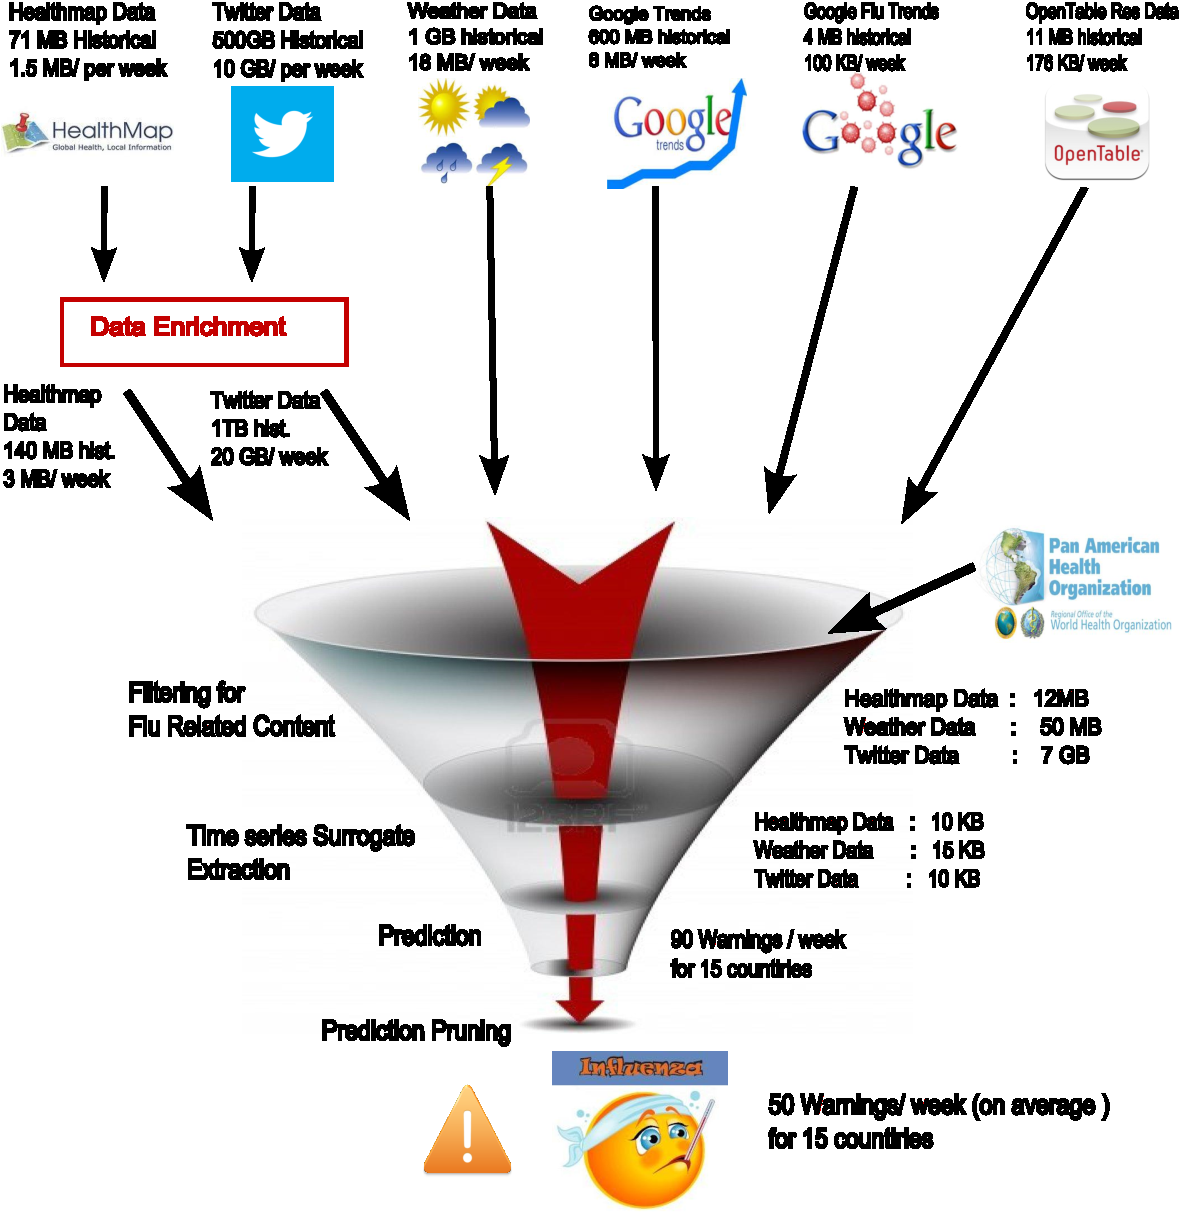
\includegraphics[scale=0.3]{fig/ili_data_pipeline.pdf}
    \caption{\label{fig:ili_data_pipeline} Different Data sources used to predict ILI case
    count values: the ``ILI Data Pipeline''}
 \end{figure}
 
 In this section, we present some of the more interesting works that have
inspired our works. We present this works into three seprate categories as follows: \\

\textbf{Keyword detection for Social Media :} 
As presented in Section~\ref{sec:intro}, there has been an work aimed at uncovering the hidden
correlations between ILI activities with social media signals from sources as diverse 
as Twitter to historical newspaper archives. Most of these methods rely on 
accurate language processing techniques and the key to such techniques is an 
accurate dictionary of ILI related keywords which we must track in order to 
uncover the relationship between the social ``chatter'' and ILI case counts. 
There has been some investigations into importance of diversity of words
in tweets ~\cite{ref5, ref6}. In
\cite{ref5}, Kanhabua and Nejdl used clustering methods to determine
important topics in Twitter data. They constructed time series for
matched keywords and used Jaccard coefficient to determine temporal
diversity of tweets. They have noted that this temporal diversity may be
correlated with real-world ILI outbreaks. On the other hand, in \cite{ref6}
authors studied the dynamic of changes in tweets related to H1N1 virus. We 
present our approach towards creating the keyword dictionary in Section~\ref{sec:keyword}.

\textbf{ Physical indicators for detecting ILI incidence levels :} 
One of the key indicators of ILI levels in a country is the prevalent 
climactic patterns and the deviation from ``normal'' levels of these 
indicators. For example Tamerius et al.~\cite{ref9}, investigated the existence of seasonal 
cycles of influenza epidemics in different climate regions
by considering
climatic information from 78 globally distributed sites. Through logistic
regression they found out that in cold-dry and humid-rainy
environments strong correlation exists between influenza epidemics and
weather conditions. Similary exciting results were found from the works
of Shaman et. al.~\cite{Shaman_orig_humidity_link, Shaman_humidity_USA}
where they found absolute humidity to be a key indicator of flu. To uncover 
these relationships they used non-linear regressors such as Kalman filters 
and this was a key inspiration to us while finding an uniform model for the
vaired data sources as explained in Section~\ref{sec:methods}.

\textbf{Non-linear regression methods}
There has been a lot of research in recommender systems to predict unknown user 
ratings from the known data using different techniques such as collaborative 
filtering, matrix factorizations and nearest neighbor detection. Although
working essentially on categorical data, these methods are fine examples of non-linear
regression methods which have been found to be robust as well as scalable (See~\cite{koren2008factor}).
While matrix factorization have been long used (see ~\cite{canny2002factor}) to 
express the independent and the dependent variables through latent factors, 
recently Koren et al.~\cite{koren2008factor} presented detailed comparisons
of nearest neighbors with matrix factorization methods and provided frameworks to 
integrate the two approaches towards an unified non-linear predictor.

\paragraph{Other Misc. Works}
Finally, there have some other related works which has helped us shape this paper. 
In \cite{ref3}, Denecke et al.
proposed an event-based approach which can be used for early prediction
of ILI threats \cite{ref3}. In their method (M-Eco) they consider
multiple resources such as Twitter, TV reports, online news articles,
and blogs. M-Eco is a bi-lingual system that works with information in
English and German and uses clustering to group documents in to
clusters. These clusters are then interpreted as signals and used for
event detection. The system is also based on supervised learning methods
that rely on signal definitions which have been entered by user.
Also, there has been some work in studying the dynamics of influenza epidemics and
modeling this behavior using dynamical systems. Network dynamic solutions are used in
\cite{ref11} to study the behavior of an epidemic issue in a society.
Spread of an infection through a network has been also studied as a
general problem in graph-mining \cite{ref13} \cite{ref14}. 
 
